\documentclass[12pt,a4paper]{article}
\usepackage{ctex}
\usepackage{amsmath,amssymb}
\usepackage{geometry}
\usepackage{booktabs}
\usepackage{graphicx}
\usepackage{float}
\usepackage{tikz}
\geometry{a4paper, left=2cm, right=2cm, top=2cm, bottom=2.5cm}
\usetikzlibrary{shapes,arrows,positioning,calc}

% 设置中文字体
\setCJKmainfont{AR PL UMing CN}
\setCJKsansfont{Noto Sans CJK SC}
\setCJKmonofont{AR PL KaitiM GB}

% 定义 TikZ 样式
\tikzstyle{block} = [rectangle, draw, fill=blue!20, text centered, rounded corners, minimum height=1.5em]
\tikzstyle{sum} = [draw, circle, minimum size=0.3cm]
\tikzstyle{output} = [coordinate]

\title{\textbf{《Robotics》第七章}}
\author{}
\date{}

\begin{document}

\maketitle

\section{机器人控制概述}

\subsection{控制问题的数学描述}

机器人控制的目标是计算执行器所需的力或力矩,以完成给定的任务。机器人动力学方程可表示为:

\begin{equation}
\boldsymbol{\tau} = \mathbf{B}(\mathbf{q})\ddot{\mathbf{q}} + \mathbf{C}(\mathbf{q},\dot{\mathbf{q}})\dot{\mathbf{q}} + \mathbf{F}_v\dot{\mathbf{q}} + \mathbf{g}(\mathbf{q})
\label{eq:robot_dynamics}
\end{equation}

其中:
\begin{itemize}
    \item $\boldsymbol{\tau}$:关节力矩向量
    \item $\mathbf{q}$:关节位置向量
    \item $\mathbf{B}(\mathbf{q})$:惯性矩阵
    \item $\mathbf{C}(\mathbf{q},\dot{\mathbf{q}})$:科里奥利力和离心力矩阵
    \item $\mathbf{F}_v$:粘性摩擦系数矩阵
    \item $\mathbf{g}(\mathbf{q})$:重力向量
\end{itemize}

\subsection{坐标系定义}

\begin{itemize}
    \item \textbf{内部坐标}:关节空间坐标 $\mathbf{q} = [q_1, q_2, \dots, q_n]^T$
    \item \textbf{外部坐标}:任务空间坐标 $\mathbf{x} = [x, y, z, \phi, \theta, \psi]^T$
    \item \textbf{正运动学}:$\mathbf{x} = \mathbf{k}(\mathbf{q})$
    \item \textbf{逆运动学}:$\mathbf{q} = \mathbf{k}^{-1}(\mathbf{x})$
\end{itemize}

\begin{figure}[H]
\centering
\begin{tikzpicture}[auto, node distance=2cm, >=stealth']
    \node[] (input) {期望轨迹 $\mathbf{x}_r$};
    \node[block, right of=input] (invkin) {逆运动学};
    \node[block, right of=invkin] (controller) {控制器};
    \node[block, right of=controller] (actuators) {执行器};
    \node[block, right of=actuators] (robot) {机器人};
    \node[block, below of=robot] (sensors) {传感器};
    \node[block, below of=invkin] (directkin) {正运动学};
    
    \node[output, right of=robot] (output) {实际轨迹 $\mathbf{x}$};
    
    \draw[->] (input) -- (invkin);
    \draw[->] (invkin) -- node {$\mathbf{q}_r$} (controller);
    \draw[->] (controller) -- node {$\mathbf{u}$} (actuators);
    \draw[->] (actuators) -- node {$\boldsymbol{\tau}$} (robot);
    \draw[->] (robot) -- (output);
    \draw[->] (robot) -- node {$\mathbf{q}$} (sensors);
    \draw[->] (sensors) -| (directkin);
    \draw[->] (directkin) -| node[pos=0.95] {$\mathbf{x}$} (controller);
\end{tikzpicture}
\caption{机器人控制系统总体结构}
\label{fig:overall_control}
\end{figure}

\section{基于内部坐标的控制}

\subsection{PD位置控制}

\subsubsection{基本PD控制}

\begin{figure}[H]
\centering
\begin{tikzpicture}[auto, node distance=1.5cm, >=stealth']
    \node[] (input) {$\mathbf{q}_r$};
    \node[sum, right of=input] (sum1) {};
    \node[block, right of=sum1] (Kp) {$\mathbf{K}_p$};
    \node[sum, right of=Kp] (sum2) {};
    \node[block, right of=sum2] (robot) {机器人};
    \node[block, below of=robot] (Kd) {$\mathbf{K}_d$};
    
    \node[output, right of=robot] (output) {$\mathbf{q}$};
    
    \draw[->] (input) -- node[pos=0.95] {$+$} (sum1);
    \draw[->] (sum1) -- node {$\tilde{\mathbf{q}}$} (Kp);
    \draw[->] (Kp) -- (sum2);
    \draw[->] (sum2) -- node {$\mathbf{u}$} (robot);
    \draw[->] (robot) -- (output);
    \draw[->] (output) |- (Kd);
    \draw[->] (Kd) -| node[pos=0.95] {$-$} (sum2);
    \draw[->] (output) -- ++(0,-2) -| node[pos=0.95] {$-$} (sum1);
\end{tikzpicture}
\caption{基本PD位置控制}
\label{fig:basic_pd}
\end{figure}

控制律:
\begin{equation}
\mathbf{u} = \mathbf{K}_p(\mathbf{q}_r - \mathbf{q}) - \mathbf{K}_d\dot{\mathbf{q}}
\label{eq:basic_pd}
\end{equation}

其中:
\begin{itemize}
    \item $\tilde{\mathbf{q}} = \mathbf{q}_r - \mathbf{q}$:位置误差
    \item $\mathbf{K}_p = \text{diag}(k_{p1}, \dots, k_{pn})$:比例增益矩阵
    \item $\mathbf{K}_d = \text{diag}(k_{d1}, \dots, k_{dn})$:微分增益矩阵
\end{itemize}

\subsubsection{改进的PD控制}

\begin{figure}[H]
\centering
\begin{tikzpicture}[auto, node distance=1.5cm, >=stealth']
    \node[] (input) {$\mathbf{q}_r$};
    \node[sum, right of=input] (sum1) {};
    \node[block, right of=sum1] (Kp) {$\mathbf{K}_p$};
    \node[sum, right of=Kp] (sum2) {};
    \node[block, above of=sum2] (Kd) {$\mathbf{K}_d$};
    \node[sum, right of=Kd] (sum3) {};
    \node[block, right of=sum2] (robot) {机器人};
    
    \node[output, right of=robot] (output) {$\mathbf{q}$};
    
    % 路径
    \draw[->] (input) -- node[pos=0.95] {$+$} (sum1);
    \draw[->] (sum1) -- node {$\tilde{\mathbf{q}}$} (Kp);
    \draw[->] (Kp) -- (sum2);
    \draw[->] (sum2) -- node {$\mathbf{u}$} (robot);
    \draw[->] (robot) -- (output);
    
    % 速度环
    \node[block, below of=input] (diff1) {$\frac{d}{dt}$};
    \draw[->] (input) -- (diff1);
    \draw[->] (diff1) -| node[pos=0.95] {$+$} (sum3);
    
    \node[block, below of=output] (diff2) {$\frac{d}{dt}$};
    \draw[->] (output) -- (diff2);
    \draw[->] (diff2) -| node[pos=0.95] {$-$} (sum3);
    
    \draw[->] (sum3) -- node {$\dot{\tilde{\mathbf{q}}}$} (Kd);
    \draw[->] (Kd) -- (sum2);
    
    \draw[->] (output) -- ++(0,-3.5) -| node[pos=0.95] {$-$} (sum1);
\end{tikzpicture}
\caption{改进的PD位置控制(包含参考速度)}
\label{fig:improved_pd}
\end{figure}

控制律:
\begin{equation}
\mathbf{u} = \mathbf{K}_p(\mathbf{q}_r - \mathbf{q}) + \mathbf{K}_d(\dot{\mathbf{q}}_r - \dot{\mathbf{q}})
\label{eq:improved_pd}
\end{equation}

\subsection{带重力补偿的PD控制}

考虑重力项的动力学方程:
\begin{equation}
\mathbf{B}(\mathbf{q})\ddot{\mathbf{q}} + \mathbf{C}(\mathbf{q},\dot{\mathbf{q}})\dot{\mathbf{q}} + \mathbf{F}_v\dot{\mathbf{q}} + \mathbf{g}(\mathbf{q}) = \boldsymbol{\tau}
\label{eq:dynamics_with_gravity}
\end{equation}

在准静态条件下($\ddot{\mathbf{q}} \approx 0$, $\dot{\mathbf{q}} \approx 0$):
\begin{equation}
\boldsymbol{\tau} \approx \mathbf{g}(\mathbf{q})
\end{equation}

\begin{figure}[H]
\centering
\begin{tikzpicture}[auto, node distance=1.5cm, >=stealth']
    \node[] (input) {$\mathbf{q}_r$};
    \node[sum, right of=input] (sum1) {};
    \node[block, right of=sum1] (Kp) {$\mathbf{K}_p$};
    \node[sum, right of=Kp] (sum2) {};
    \node[block, right of=sum2] (robot) {机器人};
    \node[block, below of=robot] (Kd) {$\mathbf{K}_d$};
    \node[block, below of=Kd] (gravity) {$\hat{\mathbf{g}}(\mathbf{q})$};
    
    \node[output, right of=robot] (output) {$\mathbf{q}$};
    
    \draw[->] (input) -- node[pos=0.95] {$+$} (sum1);
    \draw[->] (sum1) -- node {$\tilde{\mathbf{q}}$} (Kp);
    \draw[->] (Kp) -- (sum2);
    \draw[->] (sum2) -- node {$\mathbf{u}$} (robot);
    \draw[->] (robot) -- (output);
    \draw[->] (output) |- (Kd);
    \draw[->] (Kd) -| node[pos=0.95] {$-$} (sum2);
    \draw[->] (output) -- (gravity);
    \draw[->] (gravity) -| node[pos=0.95] {$+$} (sum2);
    \draw[->] (output) -- ++(0,-4) -| node[pos=0.95] {$-$} (sum1);
\end{tikzpicture}
\caption{带重力补偿的PD控制}
\label{fig:pd_gravity_compensation}
\end{figure}

控制律:
\begin{equation}
\mathbf{u} = \mathbf{K}_p(\mathbf{q}_r - \mathbf{q}) - \mathbf{K}_d\dot{\mathbf{q}} + \hat{\mathbf{g}}(\mathbf{q})
\label{eq:pd_gravity}
\end{equation}

其中 $\hat{\mathbf{g}}(\mathbf{q})$ 是重力项的估计值。

\subsection{基于逆动力学的控制}

\subsubsection{系统线性化}

定义简化动力学项:
\begin{equation}
\mathbf{n}(\mathbf{q},\dot{\mathbf{q}}) = \mathbf{C}(\mathbf{q},\dot{\mathbf{q}})\dot{\mathbf{q}} + \mathbf{F}_v\dot{\mathbf{q}} + \mathbf{g}(\mathbf{q})
\label{eq:n_term}
\end{equation}

动力学方程简化为:
\begin{equation}
\mathbf{B}(\mathbf{q})\ddot{\mathbf{q}} + \mathbf{n}(\mathbf{q},\dot{\mathbf{q}}) = \boldsymbol{\tau}
\label{eq:simplified_dynamics}
\end{equation}

直接动力学模型:
\begin{equation}
\ddot{\mathbf{q}} = \mathbf{B}^{-1}(\mathbf{q})\left(\boldsymbol{\tau} - \mathbf{n}(\mathbf{q},\dot{\mathbf{q}})\right)
\label{eq:direct_dynamics}
\end{equation}

\begin{figure}[H]
\centering
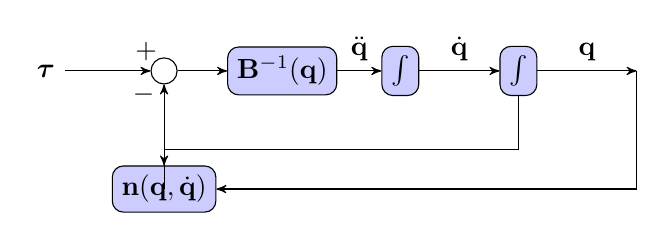
\begin{tikzpicture}[auto, node distance=1.5cm, >=stealth']
    \node[] (input) {$\boldsymbol{\tau}$};
    \node[sum, right of=input] (sum1) {};
    \node[block, right of=sum1] (Binverse) {$\mathbf{B}^{-1}(\mathbf{q})$};
    \node[block, right of=Binverse] (integral1) {$\int$};
    \node[block, right of=integral1] (integral2) {$\int$};
    \node[output, right of=integral2] (output) {$\mathbf{q}$};
    
    \node[block, below of=sum1] (nblock) {$\mathbf{n}(\mathbf{q},\dot{\mathbf{q}})$};
    
    \draw[->] (input) -- node[pos=0.95] {$+$} (sum1);
    \draw[->] (sum1) -- (Binverse);
    \draw[->] (Binverse) -- node {$\ddot{\mathbf{q}}$} (integral1);
    \draw[->] (integral1) -- node {$\dot{\mathbf{q}}$} (integral2);
    \draw[->] (integral2) -- node {$\mathbf{q}$} (output);
    
    \draw[->] (output) |- (nblock);
    \draw[->] (integral2) -- ++(0,-1) -| (nblock);
    \draw[->] (nblock) -| node[pos=0.95] {$-$} (sum1);
\end{tikzpicture}
\caption{机器人直接动力学模型}
\label{fig:direct_dynamics_model}
\end{figure}

\subsubsection{逆动力学控制律}

采用控制律:
\begin{equation}
\boldsymbol{\tau} = \hat{\mathbf{B}}(\mathbf{q})\mathbf{y} + \hat{\mathbf{n}}(\mathbf{q},\dot{\mathbf{q}})
\label{eq:inverse_dynamics_control}
\end{equation}

其中 $\hat{\mathbf{B}}(\mathbf{q})$ 和 $\hat{\mathbf{n}}(\mathbf{q},\dot{\mathbf{q}})$ 是系统模型的估计值。

\begin{figure}[H]
\centering
\begin{tikzpicture}[auto, node distance=1.5cm, >=stealth']
    \node[] (input) {$\mathbf{y}$};
    \node[block, right of=input] (Bhat) {$\hat{\mathbf{B}}(\mathbf{q})$};
    \node[sum, right of=Bhat] (sum1) {};
    \node[block, above of=sum1] (nhat) {$\hat{\mathbf{n}}(\mathbf{q},\dot{\mathbf{q}})$};
    \node[block, right of=sum1] (robot) {机器人};
    
    \node[output, right of=robot] (output) {$\mathbf{q}$};
    
    \draw[->] (input) -- (Bhat);
    \draw[->] (Bhat) -- (sum1);
    \draw[->] (nhat) -- (sum1);
    \draw[->] (sum1) -- node {$\boldsymbol{\tau}$} (robot);
    \draw[->] (robot) -- (output);
    
    \draw[->] (output) -- ++(0,-1) -| (nhat);
    \node[block, below of=nhat] (diff) {$\frac{d}{dt}$};
    \draw[->] (output) -- ++(0,-2) -| (diff);
    \draw[->] (diff) -- (nhat);
\end{tikzpicture}
\caption{基于逆动力学的控制}
\label{fig:inverse_dynamics_control}
\end{figure}

将控制律(\ref{eq:inverse_dynamics_control})代入动力学方程(\ref{eq:simplified_dynamics}):
\begin{align*}
\mathbf{B}(\mathbf{q})\ddot{\mathbf{q}} + \mathbf{n}(\mathbf{q},\dot{\mathbf{q}}) &= \hat{\mathbf{B}}(\mathbf{q})\mathbf{y} + \hat{\mathbf{n}}(\mathbf{q},\dot{\mathbf{q}}) \\
\mathbf{B}(\mathbf{q})\ddot{\mathbf{q}} &= \hat{\mathbf{B}}(\mathbf{q})\mathbf{y} + [\hat{\mathbf{n}}(\mathbf{q},\dot{\mathbf{q}}) - \mathbf{n}(\mathbf{q},\dot{\mathbf{q}})]
\end{align*}

如果模型完全准确($\hat{\mathbf{B}} = \mathbf{B}$, $\hat{\mathbf{n}} = \mathbf{n}$),则:
\begin{equation}
\ddot{\mathbf{q}} = \mathbf{y}
\label{eq:linearized_system}
\end{equation}

系统被完全线性化和解耦。

\subsubsection{闭环控制设计}

定义误差:
\begin{align}
\tilde{\mathbf{q}} &= \mathbf{q}_r - \mathbf{q} \\
\dot{\tilde{\mathbf{q}}} &= \dot{\mathbf{q}}_r - \dot{\mathbf{q}} \\
\ddot{\tilde{\mathbf{q}}} &= \ddot{\mathbf{q}}_r - \ddot{\mathbf{q}}
\end{align}

设计控制输入:
\begin{equation}
\mathbf{y} = \ddot{\mathbf{q}}_r + \mathbf{K}_p(\mathbf{q}_r - \mathbf{q}) + \mathbf{K}_d(\dot{\mathbf{q}}_r - \dot{\mathbf{q}})
\label{eq:y_design}
\end{equation}

代入线性化系统 $\ddot{\mathbf{q}} = \mathbf{y}$:
\begin{align*}
\ddot{\mathbf{q}} &= \ddot{\mathbf{q}}_r + \mathbf{K}_p(\mathbf{q}_r - \mathbf{q}) + \mathbf{K}_d(\dot{\mathbf{q}}_r - \dot{\mathbf{q}}) \\
\ddot{\mathbf{q}}_r - \ddot{\mathbf{q}} + \mathbf{K}_d(\dot{\mathbf{q}}_r - \dot{\mathbf{q}}) + \mathbf{K}_p(\mathbf{q}_r - \mathbf{q}) &= 0 \\
\ddot{\tilde{\mathbf{q}}} + \mathbf{K}_d\dot{\tilde{\mathbf{q}}} + \mathbf{K}_p\tilde{\mathbf{q}} &= 0
\label{eq:error_dynamics}
\end{align*}

这是线性二阶误差动力学方程。

\begin{figure}[H]
\centering
\begin{tikzpicture}[auto, node distance=1.2cm, >=stealth']
    % 逆动力学部分
    \node[] (yinput) {$\mathbf{y}$};
    \node[block, right of=yinput] (Bhat) {$\hat{\mathbf{B}}(\mathbf{q})$};
    \node[sum, right of=Bhat] (sum1) {};
    \node[block, above of=sum1] (nhat) {$\hat{\mathbf{n}}(\mathbf{q},\dot{\mathbf{q}})$};
    \node[block, right of=sum1] (robot) {机器人};
    
    % 位置控制部分
    \node[block, above of=yinput] (Kp) {$\mathbf{K}_p$};
    \node[block, left of=Kp] (Kd) {$\mathbf{K}_d$};
    \node[sum, left of=Kd] (sum2) {};
    \node[sum, left of=sum2] (sum3) {};
    
    % 参考输入
    \node[left of=sum3] (qr) {$\mathbf{q}_r$};
    \node[above of=sum2] (qrdot) {$\dot{\mathbf{q}}_r$};
    \node[above of=sum1] (qrddot) {$\ddot{\mathbf{q}}_r$};
    
    % 输出和反馈
    \node[output, right of=robot] (output) {$\mathbf{q}$};
    \node[block, below of=robot] (diff) {$\frac{d}{dt}$};
    
    % 连接
    \draw[->] (qr) -- node[pos=0.95] {$+$} (sum3);
    \draw[->] (sum3) -- node {$\tilde{\mathbf{q}}$} (Kp);
    \draw[->] (Kp) -- (sum2);
    \draw[->] (qrdot) -- node[pos=0.95] {$+$} (sum2);
    \draw[->] (sum2) -- (Kd);
    \draw[->] (Kd) -- (sum1);
    \draw[->] (qrddot) -- node[pos=0.95] {$+$} (sum1);
    \draw[->] (sum1) -- (Bhat);
    \draw[->] (Bhat) -- (sum1);
    \draw[->] (nhat) -- (sum1);
    \draw[->] (sum1) -- node {$\boldsymbol{\tau}$} (robot);
    \draw[->] (robot) -- (output);
    
    % 反馈路径
    \draw[->] (output) -- ++(0,-1) -| (diff);
    \draw[->] (diff) -- (nhat);
    \draw[->] (output) -- ++(0,-2.5) -| node[pos=0.95] {$-$} (sum3);
    \draw[->] (diff) -- ++(-1,0) |- node[pos=0.95] {$-$} (sum2);
\end{tikzpicture}
\caption{完整的基于逆动力学的控制系统}
\label{fig:complete_inverse_dynamics}
\end{figure}

\section{基于外部坐标的控制}

\subsection{基于雅可比转置的控制}

\subsubsection{基本原理}

从机器人静力学关系:
\begin{equation}
\boldsymbol{\tau} = \mathbf{J}^T(\mathbf{q})\mathbf{f}
\label{eq:static_relationship}
\end{equation}

其中 $\mathbf{f}$ 是末端执行器上的作用力。

控制策略:在末端执行器上虚拟地安装弹簧,产生与位置误差成正比的力:
\begin{equation}
\mathbf{f} = \mathbf{K}_p\tilde{\mathbf{x}} = \mathbf{K}_p(\mathbf{x}_r - \mathbf{x})
\label{eq:virtual_spring}
\end{equation}

\begin{figure}[H]
\centering
\begin{tikzpicture}[auto, node distance=1.5cm, >=stealth']
    \node[] (input) {$\mathbf{x}_r$};
    \node[sum, right of=input] (sum1) {};
    \node[block, right of=sum1] (Kp) {$\mathbf{K}_p$};
    \node[block, right of=Kp] (JT) {$\mathbf{J}^T(\mathbf{q})$};
    \node[block, right of=JT] (robot) {机器人};
    \node[block, below of=robot] (directkin) {$\mathbf{k}(\mathbf{q})$};
    
    \node[output, right of=robot] (output) {$\mathbf{x}$};
    
    \draw[->] (input) -- node[pos=0.95] {$+$} (sum1);
    \draw[->] (sum1) -- node {$\tilde{\mathbf{x}}$} (Kp);
    \draw[->] (Kp) -- node {$\mathbf{f}$} (JT);
    \draw[->] (JT) -- node {$\boldsymbol{\tau}$} (robot);
    \draw[->] (robot) -- (output);
    \draw[->] (robot) -- (directkin);
    \draw[->] (directkin) -| node[pos=0.95] {$-$} (sum1);
\end{tikzpicture}
\caption{基于雅可比转置的控制}
\label{fig:transposed_jacobian_control}
\end{figure}

控制律:
\begin{equation}
\boldsymbol{\tau} = \mathbf{J}^T(\mathbf{q})\mathbf{K}_p(\mathbf{x}_r - \mathbf{k}(\mathbf{q}))
\label{eq:transposed_jacobian_law}
\end{equation}

\subsection{基于逆雅可比的控制}

从微分运动学关系:
\begin{equation}
d\mathbf{x} = \mathbf{J}(\mathbf{q})d\mathbf{q} \quad \Rightarrow \quad d\mathbf{q} = \mathbf{J}^{-1}(\mathbf{q})d\mathbf{x}
\label{eq:differential_kinematics}
\end{equation}

将外部坐标误差映射到内部坐标误差:
\begin{equation}
\tilde{\mathbf{q}} = \mathbf{J}^{-1}(\mathbf{q})\tilde{\mathbf{x}}
\label{eq:error_mapping}
\end{equation}

\begin{figure}[H]
\centering
\begin{tikzpicture}[auto, node distance=1.5cm, >=stealth']
    \node[] (input) {$\mathbf{x}_r$};
    \node[sum, right of=input] (sum1) {};
    \node[block, right of=sum1] (Jinv) {$\mathbf{J}^{-1}(\mathbf{q})$};
    \node[block, right of=Jinv] (Kp) {$\mathbf{K}_p$};
    \node[block, right of=Kp] (robot) {机器人};
    \node[block, below of=robot] (directkin) {$\mathbf{k}(\mathbf{q})$};
    
    \node[output, right of=robot] (output) {$\mathbf{x}$};
    
    \draw[->] (input) -- node[pos=0.95] {$+$} (sum1);
    \draw[->] (sum1) -- node {$\tilde{\mathbf{x}}$} (Jinv);
    \draw[->] (Jinv) -- node {$\tilde{\mathbf{q}}$} (Kp);
    \draw[->] (Kp) -- node {$\boldsymbol{\tau}$} (robot);
    \draw[->] (robot) -- (output);
    \draw[->] (robot) -- (directkin);
    \draw[->] (directkin) -| node[pos=0.95] {$-$} (sum1);
\end{tikzpicture}
\caption{基于逆雅可比的控制}
\label{fig:inverse_jacobian_control}
\end{figure}

控制律:
\begin{equation}
\boldsymbol{\tau} = \mathbf{K}_p\mathbf{J}^{-1}(\mathbf{q})(\mathbf{x}_r - \mathbf{k}(\mathbf{q}))
\label{eq:inverse_jacobian_law}
\end{equation}

\subsection{外部坐标下的PD控制与重力补偿}

微分运动学关系:
\begin{equation}
\dot{\mathbf{x}} = \mathbf{J}(\mathbf{q})\dot{\mathbf{q}}
\label{eq:velocity_kinematics}
\end{equation}

控制律设计:
\begin{align}
\mathbf{f} &= \mathbf{K}_p\tilde{\mathbf{x}} - \mathbf{K}_d\dot{\mathbf{x}} \\
\boldsymbol{\tau} &= \mathbf{J}^T(\mathbf{q})\mathbf{f} + \hat{\mathbf{g}}(\mathbf{q})
\label{eq:external_pd_gravity}
\end{align}

\begin{figure}[H]
\centering
\begin{tikzpicture}[auto, node distance=1.2cm, >=stealth']
    \node[] (input) {$\mathbf{x}_r$};
    \node[sum, right of=input] (sum1) {};
    \node[block, right of=sum1] (Kp) {$\mathbf{K}_p$};
    \node[sum, right of=Kp] (sum2) {};
    \node[block, above of=sum2] (Kd) {$\mathbf{K}_d$};
    \node[block, right of=sum2] (JT) {$\mathbf{J}^T(\mathbf{q})$};
    \node[sum, right of=JT] (sum3) {};
    \node[block, right of=sum3] (robot) {机器人};
    \node[block, below of=robot] (directkin) {$\mathbf{k}(\mathbf{q})$};
    \node[block, below of=directkin] (gravity) {$\hat{\mathbf{g}}(\mathbf{q})$};
    \node[block, below of=JT] (jacobian) {$\mathbf{J}(\mathbf{q})$};
    
    \node[output, right of=robot] (output) {$\mathbf{x}$};
    
    % 主要路径
    \draw[->] (input) -- node[pos=0.95] {$+$} (sum1);
    \draw[->] (sum1) -- node {$\tilde{\mathbf{x}}$} (Kp);
    \draw[->] (Kp) -- (sum2);
    \draw[->] (sum2) -- node {$\mathbf{f}$} (JT);
    \draw[->] (JT) -- (sum3);
    \draw[->] (sum3) -- node {$\boldsymbol{\tau}$} (robot);
    \draw[->] (robot) -- (output);
    
    % 速度反馈
    \node[block, below of=Kp] (diff) {$\frac{d}{dt}$};
    \draw[->] (output) |- (diff);
    \draw[->] (diff) -| node[pos=0.95] {$-$} (Kd);
    \draw[->] (Kd) -- (sum2);
    
    % 重力补偿
    \draw[->] (robot) -- (directkin);
    \draw[->] (directkin) -- (gravity);
    \draw[->] (gravity) -| node[pos=0.95] {$+$} (sum3);
    
    % 雅可比计算
    \draw[->] (robot) -- ++(0,-4) -| (jacobian);
    \node[block, left of=jacobian] (diff2) {$\frac{d}{dt}$};
    \draw[->] (robot) -- ++(0,-5) -| (diff2);
    \draw[->] (diff2) -- (jacobian);
    
    \draw[->] (directkin) -| node[pos=0.95] {$-$} (sum1);
\end{tikzpicture}
\caption{外部坐标下的PD控制与重力补偿}
\label{fig:external_pd_gravity}
\end{figure}

\subsection{外部坐标下的逆动力学控制}

\subsubsection{加速度关系}

对速度关系(\ref{eq:velocity_kinematics})求导:
\begin{equation}
\ddot{\mathbf{x}} = \mathbf{J}(\mathbf{q})\ddot{\mathbf{q}} + \dot{\mathbf{J}}(\mathbf{q},\dot{\mathbf{q}})\dot{\mathbf{q}}
\label{eq:acceleration_kinematics}
\end{equation}

定义外部坐标误差:
\begin{align}
\tilde{\mathbf{x}} &= \mathbf{x}_r - \mathbf{x} \\
\dot{\tilde{\mathbf{x}}} &= \dot{\mathbf{x}}_r - \dot{\mathbf{x}} \\
\ddot{\tilde{\mathbf{x}}} &= \ddot{\mathbf{x}}_r - \ddot{\mathbf{x}}
\end{align}

设计误差动力学:
\begin{equation}
\ddot{\tilde{\mathbf{x}}} + \mathbf{K}_d\dot{\tilde{\mathbf{x}}} + \mathbf{K}_p\tilde{\mathbf{x}} = 0
\label{eq:external_error_dynamics}
\end{equation}

解得:
\begin{equation}
\ddot{\mathbf{x}} = \ddot{\mathbf{x}}_r + \mathbf{K}_d\dot{\tilde{\mathbf{x}}} + \mathbf{K}_p\tilde{\mathbf{x}}
\label{eq:external_acceleration}
\end{equation}

\subsubsection{控制律推导}

由方程(\ref{eq:acceleration_kinematics}):
\begin{equation}
\ddot{\mathbf{q}} = \mathbf{J}^{-1}(\mathbf{q})(\ddot{\mathbf{x}} - \dot{\mathbf{J}}(\mathbf{q},\dot{\mathbf{q}})\dot{\mathbf{q}})
\label{eq:joint_acceleration}
\end{equation}

代入(\ref{eq:external_acceleration}):
\begin{equation}
\mathbf{y} = \mathbf{J}^{-1}(\mathbf{q})(\ddot{\mathbf{x}}_r + \mathbf{K}_d\dot{\tilde{\mathbf{x}}} + \mathbf{K}_p\tilde{\mathbf{x}} - \dot{\mathbf{J}}(\mathbf{q},\dot{\mathbf{q}})\dot{\mathbf{q}})
\label{eq:external_y}
\end{equation}

完整的控制律:
\begin{equation}
\boldsymbol{\tau} = \hat{\mathbf{B}}(\mathbf{q})\mathbf{y} + \hat{\mathbf{n}}(\mathbf{q},\dot{\mathbf{q}})
\label{eq:complete_external_control}
\end{equation}

其中 $\mathbf{y}$ 由方程(\ref{eq:external_y})给出。

\section{接触力控制}

\subsection{与环境交互的动力学}

当机器人与环境接触时,动力学方程为:
\begin{equation}
\mathbf{B}(\mathbf{q})\ddot{\mathbf{q}} + \mathbf{n}(\mathbf{q},\dot{\mathbf{q}}) = \boldsymbol{\tau} - \mathbf{J}^T(\mathbf{q})\mathbf{f}
\label{eq:contact_dynamics}
\end{equation}

其中 $\mathbf{f}$ 是接触力。

\subsection{基于逆动力学的线性化}

采用控制律:
\begin{equation}
\boldsymbol{\tau} = \hat{\mathbf{B}}(\mathbf{q})\mathbf{y} + \hat{\mathbf{n}}(\mathbf{q},\dot{\mathbf{q}}) + \mathbf{J}^T(\mathbf{q})\mathbf{f}
\label{eq:force_control_law}
\end{equation}

代入动力学方程(\ref{eq:contact_dynamics}):
\begin{align*}
\mathbf{B}(\mathbf{q})\ddot{\mathbf{q}} + \mathbf{n}(\mathbf{q},\dot{\mathbf{q}}) &= \hat{\mathbf{B}}(\mathbf{q})\mathbf{y} + \hat{\mathbf{n}}(\mathbf{q},\dot{\mathbf{q}}) + \mathbf{J}^T(\mathbf{q})\mathbf{f} - \mathbf{J}^T(\mathbf{q})\mathbf{f} \\
\mathbf{B}(\mathbf{q})\ddot{\mathbf{q}} &= \hat{\mathbf{B}}(\mathbf{q})\mathbf{y} + [\hat{\mathbf{n}}(\mathbf{q},\dot{\mathbf{q}}) - \mathbf{n}(\mathbf{q},\dot{\mathbf{q}})]
\end{align*}

如果模型准确,则 $\ddot{\mathbf{q}} = \mathbf{y}$,系统被线性化。

\subsection{力控制策略}

将力控制问题转化为位置控制问题。设计虚拟系统:
\begin{equation}
\mathbf{f} = \mathbf{B}_c\ddot{\mathbf{x}}_c + \mathbf{F}_c\dot{\mathbf{x}}_c
\label{eq:virtual_system}
\end{equation}

其中:
\begin{itemize}
    \item $\mathbf{f} = \mathbf{f}_r - \mathbf{f}$:力误差
    \item $\mathbf{B}_c$:虚拟惯性矩阵
    \item $\mathbf{F}_c$:虚拟阻尼矩阵
\end{itemize}

解得虚拟运动:
\begin{equation}
\ddot{\mathbf{x}}_c = \mathbf{B}_c^{-1}(\mathbf{f} - \mathbf{F}_c\dot{\mathbf{x}}_c)
\label{eq:virtual_motion}
\end{equation}

通过积分得到虚拟位置 $\mathbf{x}_c$ 和速度 $\dot{\mathbf{x}}_c$。

\subsection{并行组合控制}

同时控制位置和力:
\begin{align}
\mathbf{x}_r &= \mathbf{x}_d + \mathbf{x}_c \\
\dot{\mathbf{x}}_r &= \dot{\mathbf{x}}_d + \dot{\mathbf{x}}_c \\
\ddot{\mathbf{x}}_r &= \ddot{\mathbf{x}}_d + \ddot{\mathbf{x}}_c
\end{align}

其中:
\begin{itemize}
    \item $\mathbf{x}_d, \dot{\mathbf{x}}_d, \ddot{\mathbf{x}}_d$:期望的位置轨迹
    \item $\mathbf{x}_c, \dot{\mathbf{x}}_c, \ddot{\mathbf{x}}_c$:由力控制产生的修正轨迹
\end{itemize}

\begin{figure}[H]
\centering
\begin{tikzpicture}[auto, node distance=1.2cm, >=stealth']
    % 力控制器
    \node[] (fr) {$\mathbf{f}_r$};
    \node[sum, right of=fr] (sumf) {};
    \node[block, right of=sumf] (forcectrl) {力控制器};
    \node[block, right of=forcectrl] (integral1) {$\int$};
    \node[block, right of=integral1] (integral2) {$\int$};
    
    % 位置控制器
    \node[above of=fr] (xd) {$\mathbf{x}_d$};
    \node[above of=sumf] (sumx) {};
    
    % 并行组合
    \node[sum, right of=integral2] (sum1) {};
    \node[sum, above of=sum1] (sum2) {};
    \node[sum, above of=sum2] (sum3) {};
    
    % 主控制器
    \node[block, right of=sum1] (posctrl) {位置控制};
    \node[block, right of=posctrl] (invdyn) {逆动力学};
    \node[block, right of=invdyn] (robot) {机器人};
    
    % 输出和反馈
    \node[output, right of=robot] (output) {$\mathbf{x}$};
    \node[block, below of=robot] (force_sensor) {力传感器};
    
    % 连接
    \draw[->] (fr) -- node[pos=0.95] {$+$} (sumf);
    \draw[->] (sumf) -- node {$\tilde{\mathbf{f}}$} (forcectrl);
    \draw[->] (forcectrl) -- node {$\ddot{\mathbf{x}}_c$} (integral1);
    \draw[->] (integral1) -- node {$\dot{\mathbf{x}}_c$} (integral2);
    \draw[->] (integral2) -- node {$\mathbf{x}_c$} (sum1);
    
    \draw[->] (xd) -| (sum3);
    \draw[->] (sum3) -- node {$\ddot{\mathbf{x}}_r$} (sum2);
    \draw[->] (sum2) -- node {$\dot{\mathbf{x}}_r$} (sum1);
    \draw[->] (sum1) -- node {$\mathbf{x}_r$} (posctrl);
    
    \draw[->] (posctrl) -- node {$\mathbf{y}$} (invdyn);
    \draw[->] (invdyn) -- node {$\boldsymbol{\tau}$} (robot);
    \draw[->] (robot) -- (output);
    
    \draw[->] (robot) -- (force_sensor);
    \draw[->] (force_sensor) -| node[pos=0.95] {$-$} (sumf);
    
    % 内部连接
    \draw[->] (integral1) -- ++(0,1) -| (sum2);
    \draw[->] (integral2) -- ++(0,2) -| (sum3);
\end{tikzpicture}
\caption{并行组合力控制系统}
\label{fig:parallel_force_control}
\end{figure}


\end{document}